\begin{center}
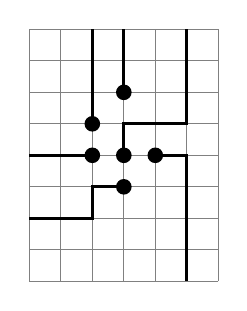
\begin{tikzpicture}[ thick, every node/.style={scale=1},level distance=1.7cm, sibling distance=2cm]

  \draw[step=0.4cm,thin, gray] (0, 0) grid (2.4, 3.2);

  \node[circle, fill=black, inner sep=0.7mm] at (1.2, 1.2) {};
  \draw[very thick] (1.2, 1.2) -- (0.8, 1.2) -- (0.8, 0.8) -- (0.0, 0.8);

  \node[circle, fill=black, inner sep=0.7mm] at (0.8, 1.6) {};
  \draw[very thick] (0.8, 1.6) -- (0.4, 1.6) -- (0.0, 1.6);

  \node[circle, fill=black, inner sep=0.7mm] at (1.6, 1.6) {};
  \draw[very thick] (1.6, 1.6) -- (2.0, 1.6) --  (2.0, 0);

  \node[circle, fill=black, inner sep=0.7mm] at (1.2, 2.4) {};
  \draw[very thick] (1.2, 2.4) -- (1.2, 3.2);

  \node[circle, fill=black, inner sep=0.7mm] at (0.8, 2) {};
  \draw[very thick] (0.8, 2) -- (0.8, 3.2);

  \node[circle, fill=black, inner sep=0.7mm] at (1.2, 1.6) {};
  \draw[very thick] (1.2, 1.6) -- (1.2, 2) -- (2, 2) -- (2, 3.2);



\end{tikzpicture}
\end{center}
